\chapter[ROSDashboard: A Visual Debugging System for ROS]{ROSDashboard: A Visual\\Debugging System for ROS}
\label{rosdashboard}

ROSDashboard is a prototypical implementation of the system designed in Chapter~\ref{visual_debugging_system}. The implementation makes use of the ROS publish/subscribe communication infrastructure to gather data and visualizes the data published by the respective ROS nodes. The data can be taken either from existing node-to-node communication or from explicit logging statements that publish data for visualization only.

Although the design in Chapter~\ref{visual_debugging_system} does not imply the use of a specific robotic framework, some of the architectural decisions were driven by the ROS architecture which was examined during the initial survey of existing debugging tools and practices in robotics. Especially the callback-style to get new values from the communication middleware to the user interface (see Figure~\ref{update_value_sequence}) was inspired by ROS. As a result, the implementation of ROSDashboard did not require a lot of glue code to connect to the communication infrastructure. If another robotic framework is chosen as target platform for an implementation, more work might be required to access the data from the robotic application. This highly depends on the existing communication infrastructure of such a robotic framework and whether it can be accessed transparently without the robot module knowing about the visualization.

This chapter gives a detailed introduction to ROS with the tools related to debugging and visualization, which influenced the development of ROSDashboard. The second section in this chapter presents ROSDashboard's implementation details, ranging from the user interface level down to the ROSDashboard API and the topic introspection that makes the use of ROSDashboard easier.

%[Not sure if this is possible in other frameworks, if not it could be stated that more work is needed for those frameworks in order to make communication transparent. In general I can argue that ROS fits the requierements best, the system design was not intended to fit every framework but was developed without compromises current systems might have]

%[I'm not sure how to write this chapter: can I have a section "why ROS?", "how the requirements are met?", ...?] ---> this should be written in the introduction for this chapter: ROS was used because it has many users, an easily accesible communication structure, a tool landscape (?) where such a tool would fit in well (recent surge of graphical tools like rxdeveloper, rqt, other dashboards).

%[from icra]
%ROSDashboard, the tool presented in this work, aims to support the developer during debugging by visualizing data in a graphic way and thus eliminating the cognitive effort needed to parse and interpret text based logging messages. While most of the currently available visualization tools in robotics focus on spatial data to help understand the robot and the environment in which it runs \cite{Collett2010, Quigley2009}, rendering of abstract data is still uncommon. ROSDashboard provides a dashboard interface to robot developers, which they can populate with graphical widgets to visualize all kinds of data from the robot. The dashboard can be customized to display widgets according to the current robot hardware and development stage. It can be used to visualize data during debugging as well as monitor data during the normal execution of the robot. This means ROSDashboard is a tool that a) can be adapted to many different use cases and b) allows the developer to choose the widgets he or she thinks represent the data best, according to their mental model and the meaning of the data. The tool is based on ROS (Robot Operating System) which abstracts from specific robot hardware and takes care of inter process communication \cite{Quigley2009}.


%%%%% Robot Operating System ROS %%%%%%
\section{ROS (Robot Operating System)}
\label{ros_overview}
The ROS (Robot Operating System) is an Open Source framework for complex robotic systems. The first work on ROS was done as part of the STanford Artificial Intelligence Robot (STAIR) in 2007 \cite{Quigley2007}. The original software library was called \emph{Switchyard} and had been developed at Stanford University. Later the library was refined and generalized to also suit the requirements of the Personal Robot Program at Willow Garage\footnote{www.willowgarage.com} \cite{Quigley2009}. The resulting general framework has been released as Open Source \cite{Quigley2009} and this section gives a short overview of the most important principles in ROS.

\begin{figure}[ht]
\centering
\subfigure[Stanford's STAIR]{
	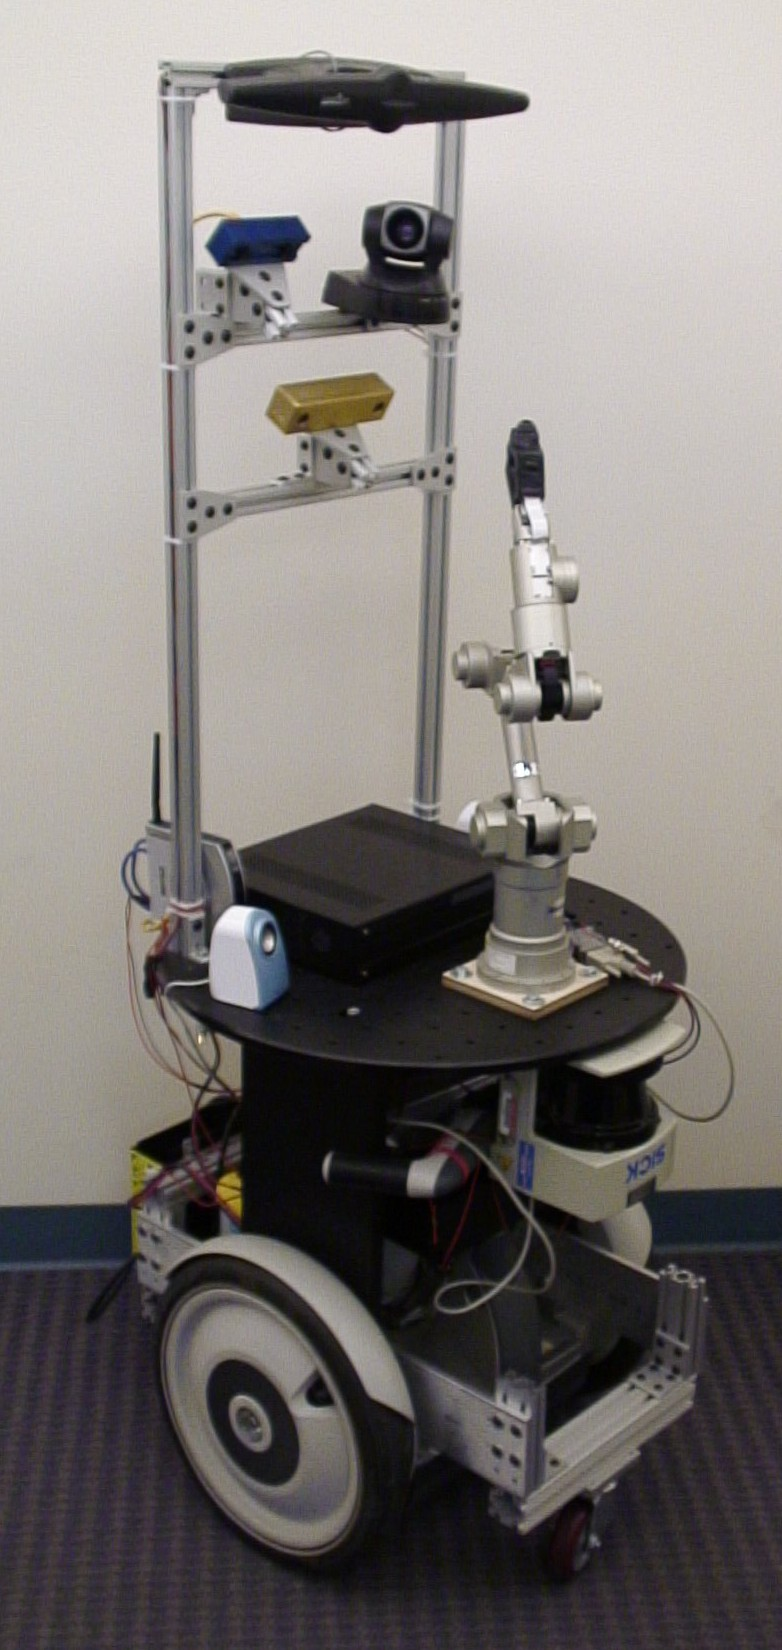
\includegraphics[height=8cm]{img/stair}
}
\subfigure[Willow Garage's PR2]{
	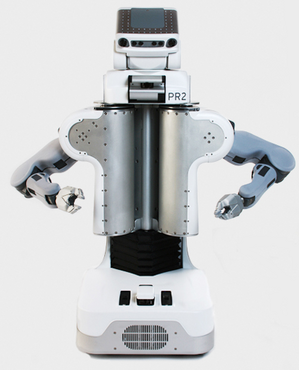
\includegraphics[height=8cm]{img/pr2}
}
\end{figure}

ROS has grown significantly in the last years with an active community backing the project and the support for many of the currently available robots \cite{Foote2012}. It was developed to abstract from the hardware of the robot and make it easier to create modular robot software which can run on different robots and on different machines. The modular approach makes development easier, because the work can be divided amongst different developers or development teams. This also allows the developer to change only small parts of a complex system, without the need to build and re-deploy the whole system.
The modules in ROS are called \emph{nodes} and several nodes executed together are called a \emph{stack}. ROS \emph{packages} bundle nodes and stacks and are used to make software modules available to other developers. Everyone can create their own package which can be indexed by ROS so that their software modules can be found, downloaded and used by other developers. There are many packages, nodes and stacks available bundling implementations of algorithms for some of the most common problems in robotics (e.g. navigation, localization, joint movement, etc.) and they can easily be (re-)used \cite{Cousins2010}.

The communication between ROS nodes is either asynchronous through a publish/subscribe mechanism or synchronous through services. With the asynchronous approach nodes can send messages by publishing a message on a topic and receive messages by subscribing to that topic. This mechanism is flexible and decouples the sender from the receiver: A publisher node does not need to know if there are other nodes listening and vice versa. The routing for those publish/subscribe messages is established during runtime through the ROS core. For synchronous communication and guaranteed delivery of messages, services can be invoked. Since the communication with services couples the sender to the receiver, services were not a relevant data source for ROSDashboard. The communication between nodes is one of the main sources for debugging data when debugging a ROS application. The same communication framework is also used for the logging mechanism in ROS, which publishes messages to the special purpose topic \emph{/rosout} (see Section~\ref{ros_logging}).

ROS was chosen as a target platform because it has become a stable and popular robotic framework in recent years \cite{Foote2012}. Many tutorials and code samples made it easy to learn how to program for ROS and the ROS community was helpful and quick to respond if questions arose during the implementation of ROSDashboard. This includes help for ROS beginners as well as valuable feedback on the design and implementation of ROSDashboard. The publish/subscribe mechanism in ROS provides an easy communication layer that can be accessed using the ROS client API. This communication style allows ROSDashboard to easily connect the visualization widgets to the data source without the source knowing about the visualization. Since ROS is a modular framework and encourages to encapsulate functionality in several small nodes rather then a single big node, the data on communication channels between existing nodes can be accessed and visualized. ROSDashboard fits well into the existing ROS tool suite and fills the gap between visualization of complex data in RViz (see Section~\ref{rviz}) and text only debugging with the ROS logging mechanism (see Section~\ref{ros_logging}). This section presents further ROS tools which were not introduced in Chapter~\ref{debugging_in_robotics} since they are not debugging specific.

\subsection{Related ROS Tools}
While most of the initial tools developed for ROS were mostly command line based, many graphical tools have been developed recently. This surge of graphical tools shows that ROS has become more wide spread and developers started working on ROS projects which are probably not as familiar with command line tools as the core developers of ROS are. Most of the graphical tools were created to help developers understand the data flowing back and forth between modules and the topics through which the data was transported. This section only presents the tools which were not already introduced in Chapter~\ref{debugging_in_robotics}.

\texttt{rxplot} is a graphical tool which can plot values from topics on a Cartesian coordinate system (see Figure~\ref{rxplot_screenshot}. The tool takes data from a published ROS topic and prints it on a time graph. The tool can be configured to visualize several graphs in one go, which makes it easy to compare values and data streams.

\begin{figure}[h]
  \centering
  \framebox{
    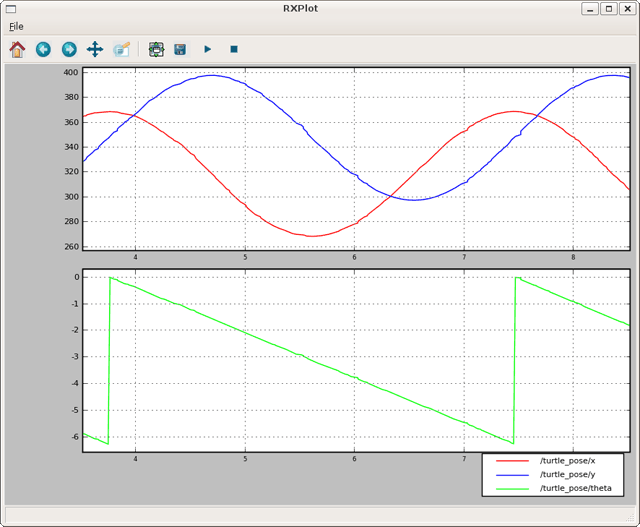
\includegraphics[width=0.55\textwidth]{img/rxplot_screenshot.png}
  }  
  \caption{rxplot screenshot. Available under a CC BY 3.0 license at \url{http://www.ros.org/wiki/rxplot}}
  \label{rxplot_screenshot}
\end{figure}

\texttt{rxconsole} provides a graphical interface for logging messages. ROS logging messages are published on the special purpose topic \emph{/rosout} and can be viewed either with a normal console or with the graphical rxconsole interface. The graphical interface can filter logging messages by text and by severity (see Figure~\ref{rxconsole_screenshot}).\enlargethispage{-2em}

\begin{figure}[p]
  \centering
  \framebox{
    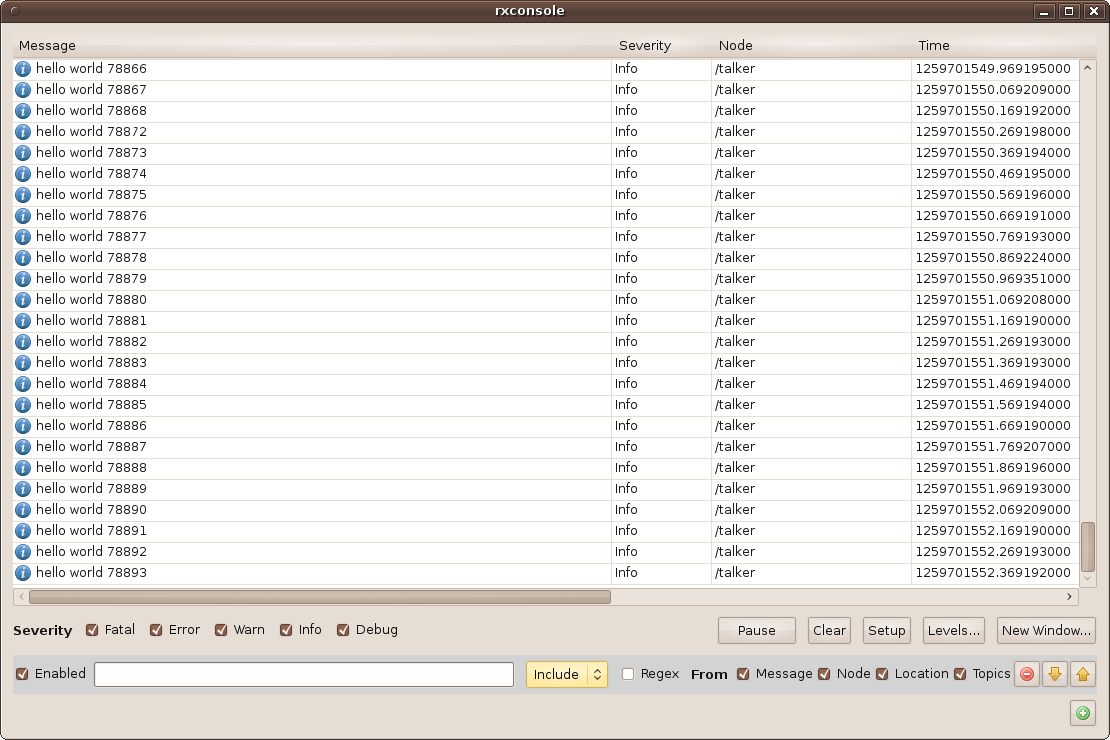
\includegraphics[width=0.8\textwidth]{img/rxconsole_screenshot.png}
  }  
  \caption{rxconsole screenshot. Available under a CC BY 3.0 license at \url{http://www.ros.org/wiki/rxconsole}}
  \label{rxconsole_screenshot}
\end{figure}


\begin{figure}[p]
  \centering
  \framebox{
    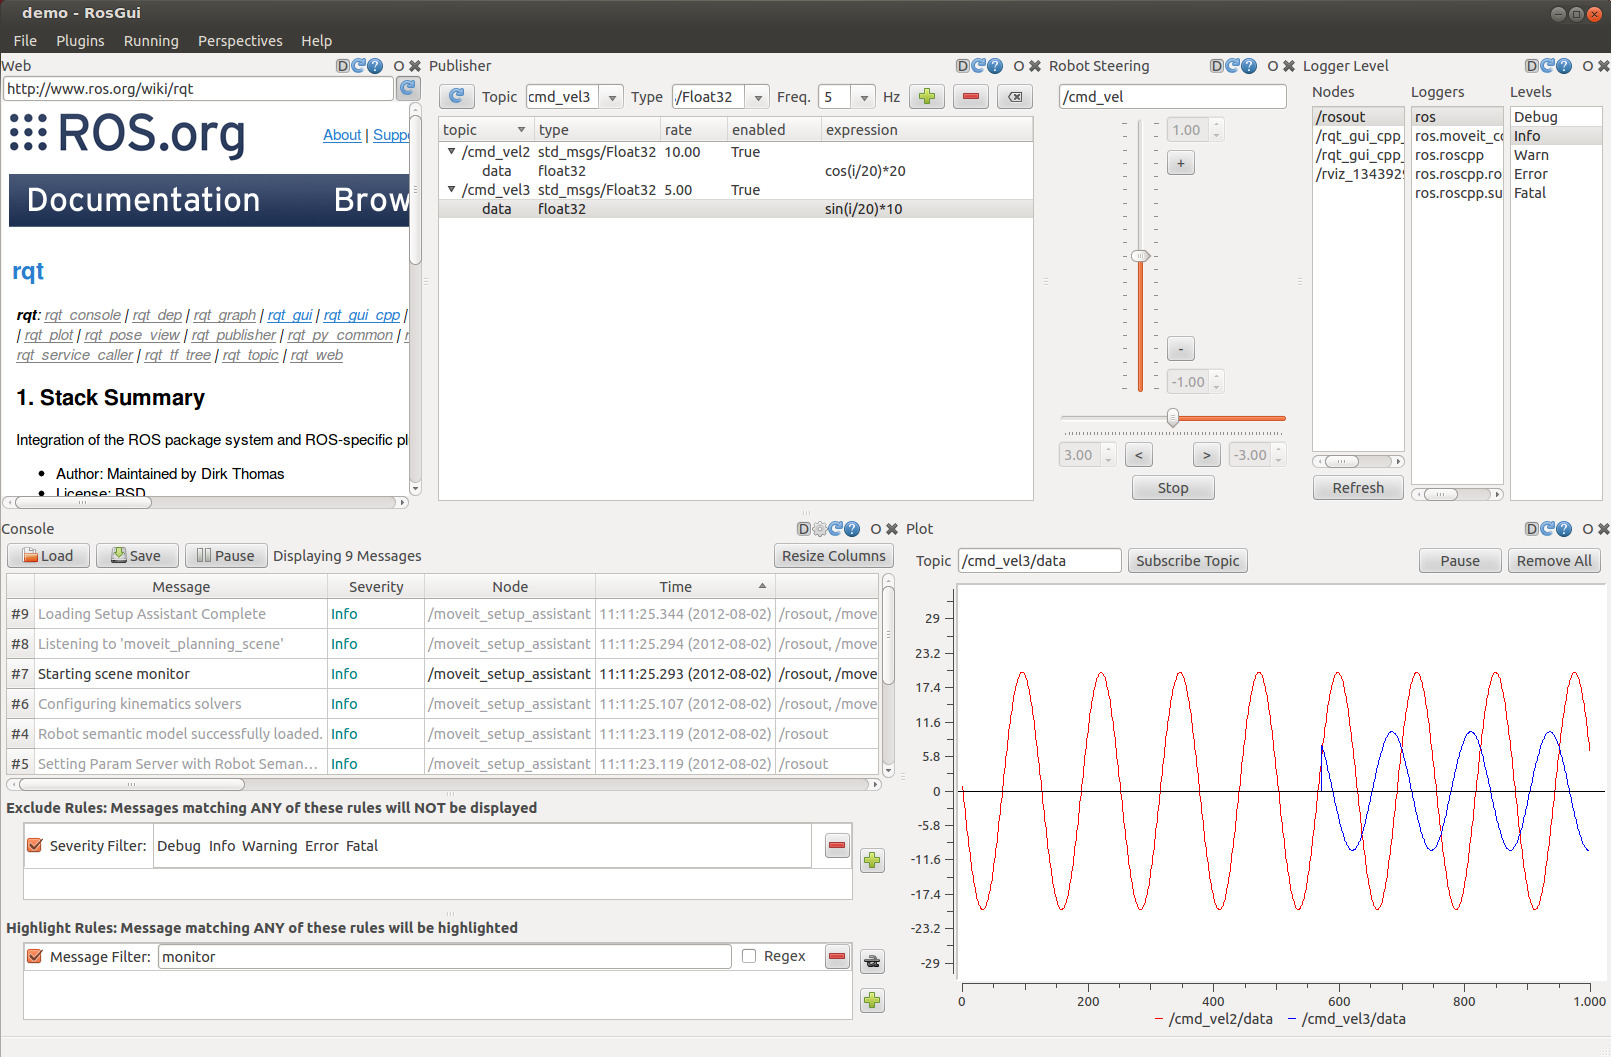
\includegraphics[width=0.8\textwidth]{img/rqt_screenshot.png}
  }  
  \caption{rqt screenshot. Available under a CC BY 3.0 license at \url{http://www.ros.org/wiki/rqt}}
  \label{rqt_screenshot}
\end{figure}

\texttt{rqt} (formerly rosgui) is a project that aims to unify the graphical user interface for ROS tools. It provides a hull where other tools can be loaded through plugins (see Figure~\ref{rqt_screenshot}). rqt's interface is based on the Qt window toolkit which is currently the recommended window toolkit for ROS. The interface provides a single point of access to all other graphical ROS tools by exposing them as plugins. The plugins can be enabled and positioned inside rqt. This allows developers to create perspectives for special use cases, where a set of graphical ROS tools are used. rqt manages the life cycle of the plugins by exposing a plugin API which has to be implemented by every plugin. When a perspective is saved the configuration of every plugin is saved as well. This makes it easy to pick up work where left off.

ROSDashboard fills the gap between highly sophisticated visualizations in \texttt{RViz} and \texttt{rxplot}, which only offers one kind of visualization. It distinguishes itself from other graphical tools by giving the developers full flexibility to choose themselves what visualization they prefer. \texttt{rqt} aims to bring together all the different graphical tools in ROS. ROSDashboard deliberately does not offer a record and replay functionality, since this is the main functionality of \texttt{rosbag}. ROSDashboard can be combined with \texttt{rosbag} in \texttt{rqt} to give developers the possibility to use record and replay together with visualizations. Although \texttt{rxbag} already contains some support for visualizations, it mainly focuses on replaying data and looking at data in detail after the execution has stopped. This distinguishes \texttt{rxbag} from ROSDashboard, which focuses on visualizations during the execution of a program.

%\texttt{rxDeveloper}

%\subsubsection{rxDeveloper}
%[\textbf{outline, results of the survey, importance for this work}]
%\cite{Muellers2012}

%\todo{list some tools and recent projects that have influenced the tool. For example the rxdeveloper tool and the survey in Muellers2012, RQT and other dashboards recently developed. Highly related to the choice of making a tool for ros.}

%%%%% Implementation Details %%%%%%
\section{Implementation Details}
This section presents the implementation details of ROSDashboard. The first part shows in detail how the visualization widgets are connected to a ROS topic and what difficulties had to be resolved. Part two of this section presents the user interface details and shows screenshots of ROSDashboard in action. The third part introduces the data format in which dashboards can be saved and restored from a file. The ROSDashboard API is a set of convenience methods to publish data on topics and is shown in the last part.

\subsection{Topic Introspection}

\begin{figure}[thpb]
  \centering
  \framebox{
    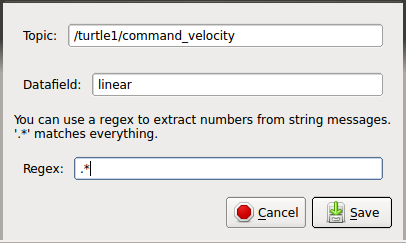
\includegraphics[scale=0.8]{img/topic_setup_2.png}
  }  
  \caption{Screenshot of the topic setup dialog.}
  \label{topic setup screenshot}
\end{figure}

ROS topics were originally not designed and developed as something the user or developer chooses graphically: They are usually created, configured and used in the source code. ROSDashboard exposes the topic setup in a graphical user interface every time a new widget is added to the dashboard. To make this as easy as possible and without much overhead, a technical solution was chosen to reduce the number of fields to be set during the topic subscription setup. Normally you have to select a topic name and a message data type. The data type can be one of the standard message types like Float, Integer, String and Boolean or a more complex message type which contains more information in a structured message. To access one data element of a message the ``datafield'' field was introduced in the graphical interface. Figure~\ref{topic setup screenshot} shows an exemplary topic setup configuration to access the linear velocity of the \emph{/turtlesim/Velocity} message published to the topic \emph{/turtle1/command\_velocity}. Using Python's duck typing and the \emph{rostopic} module it was possible to avoid the complexity of dynamically binding message type classes during runtime and detect the message type automatically. If a topic is not yet published and thus the message type of this topic is not defined yet, the method call to \emph{rostopic} will block until the message type becomes available. To avoid blocking of the user interface a listener thread was implemented to wait until the message type for a topic becomes available (see Figure~\ref{topic subscription}). Avoiding to manually ask the user for a message type makes the configuration of widgets easier and faster for the user, it also keeps the implementation significantly simpler, because no dynamic binding of message type classes during runtime is needed.

\begin{figure}[thpb]
  \centering
  \framebox{
    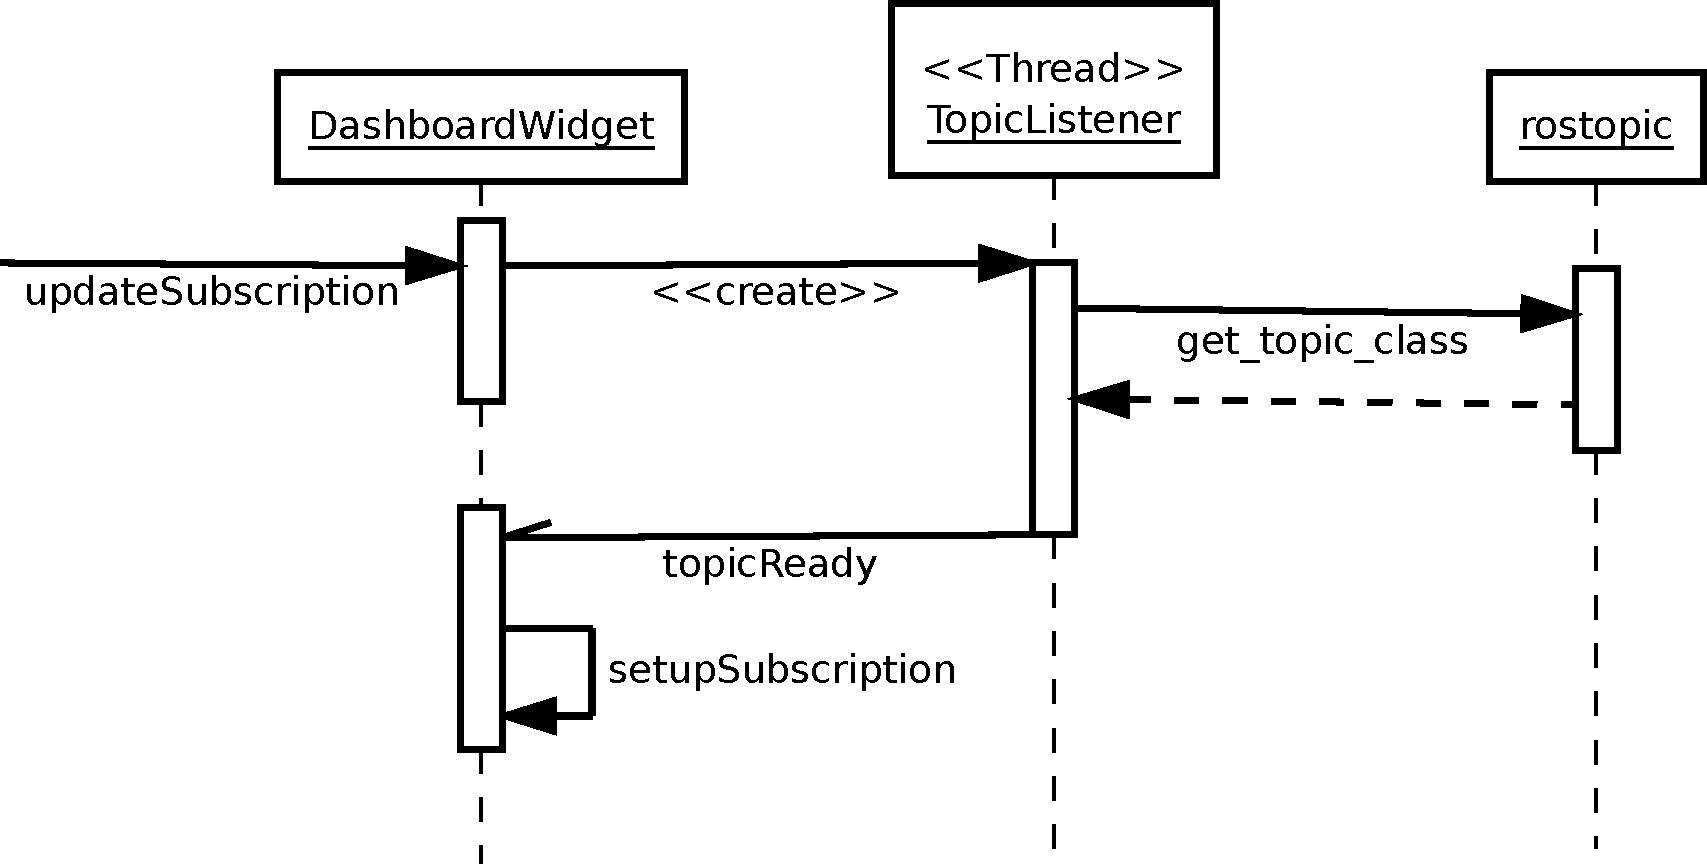
\includegraphics[scale=0.4]{diagrams/topic_subscription.pdf}
  }  
  \caption{Exemplary flow of events for asynchronous topic subscription setup.}
  \label{topic subscription}
\end{figure}

\subsection{Transparent Data Collection with Regular Expressions}
\label{transparent_collection}

Figure~\ref{topic setup screenshot} shows a third field in the user interface to set up a topic subscription. The ``Regex'' field can be used to apply a regular expression on a message to filter the message or extract numerical data from a String message. As mentioned in Section~\ref{ros_logging}, the logging messages in ROS are String messages. Those messages often contain numerical data which can currently not be used for visualization because of the lack of type information. Since many existing ROS modules make extensive use of the logging framework it is important to provide access to this information. The regular expression gives developers transparent access to the data embedded in logging messages, without the need to have access to and modify the source code of a module they want to debug.

The code to check the regular expression is contained in the \textbf{Adapter} class, which parses the value it receives in the \verb+callback()+ method from the communication middleware (see Figure~\ref{update_value_sequence}). This hides the regular expression handling from the \textbf{DashboardWidget} and \textbf{ConcreteVisualizationWidget} (see Figure~\ref{class overview}). The widget can thus focus on the graphical part and expect polished data which can be visualized straight away, without further pre-processing. Encapsulating the regular expression matching in the \textbf{Adapter} means future plugin developers do not need to care about the regular expression handling unless they want to, in which case they can overwrite the subscription setup methods in their visualization widget implementation to circumvent the integrated regular expression evaluation.

\subsection{User Interface}
The user interface was implemented based on the early interface designs from Section~\ref{graphical_user_interface}. The main window consists of the dashboard canvas where visualization widgets can be positioned freely and a toolbox where all the available visualization widgets can be selected. The visualization widgets can be positioned on the dashboard by ``Drag\&Drop'' from the toolbox. Figure~\ref{screenflow} shows a series of screenshots, depicting every step necessary to put a visualization widget on the dashboard: First the desired widget needs to be selected in the toolbox and dragged to the dashboard. When the widget is dropped on the dashboard, the configuration dialog opens automatically where the developer can select to which topic and datafield the visualization widget should connect to. This dialog can be re-opened later from the context menu of the widget, as well as the rename dialog and the properties dialog. It was deliberately chosen to separate the dialog for setting up a topic connection and the dialog for other settings of the widget. This separation of concerns keeps the data provider setup encapsulated in its own dialog, which makes it easier to exchange the data provider if necessary. To remove a widget from the dashboard, simply drag it to the bottom of the dashboard where a special drop zone deletes the widget from the dashboard.

\begin{figure}[p]
\centering
\subfigure[Empty dashboard]{
    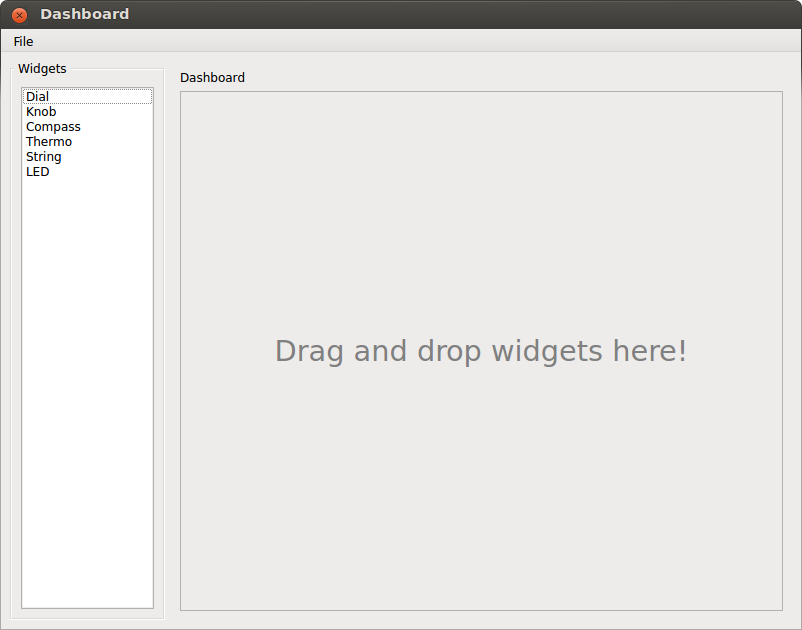
\includegraphics[width=0.45\textwidth]{img/screenflow1.png}
}
\subfigure[Dragging widget to dashboard]{
    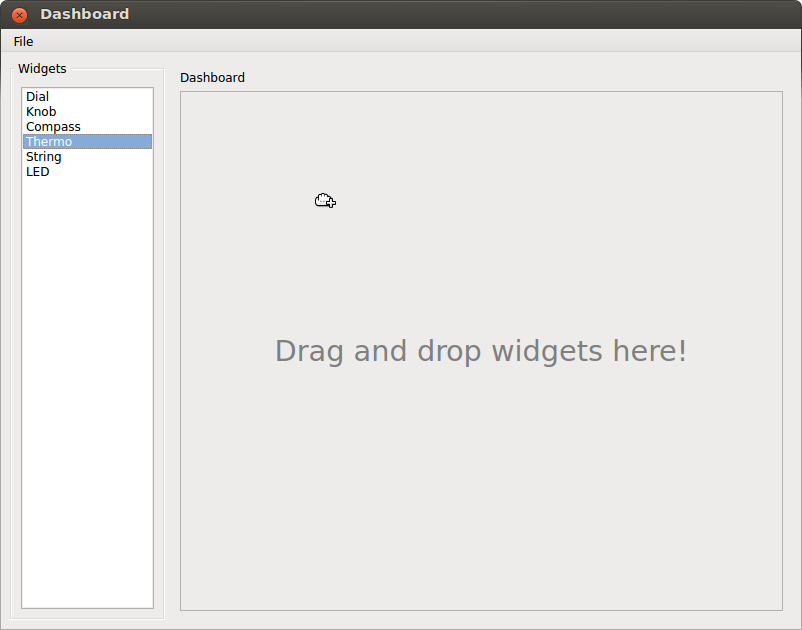
\includegraphics[width=0.45\textwidth]{img/screenflow2.png}
}
\subfigure[Configure subscription on drop]{
    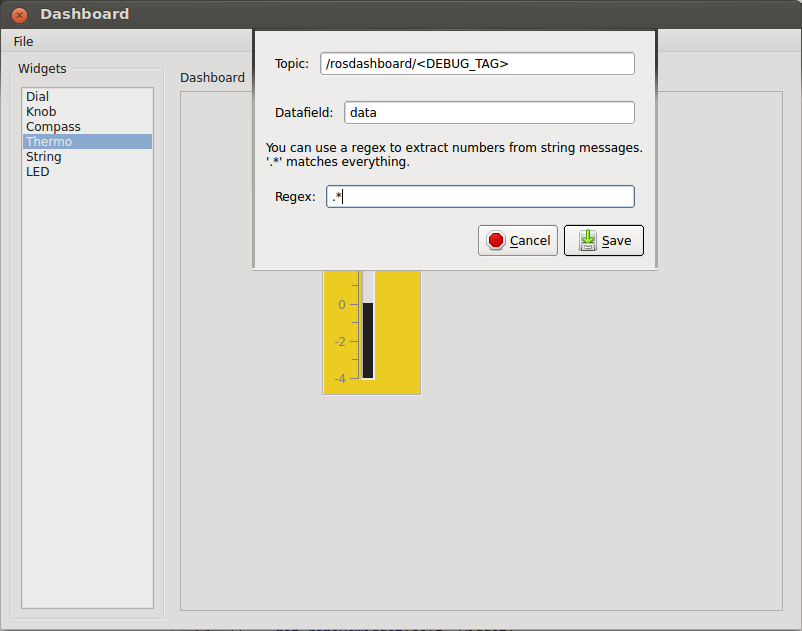
\includegraphics[width=0.45\textwidth]{img/screenflow3_2.png}
}
\subfigure[Context menu]{
    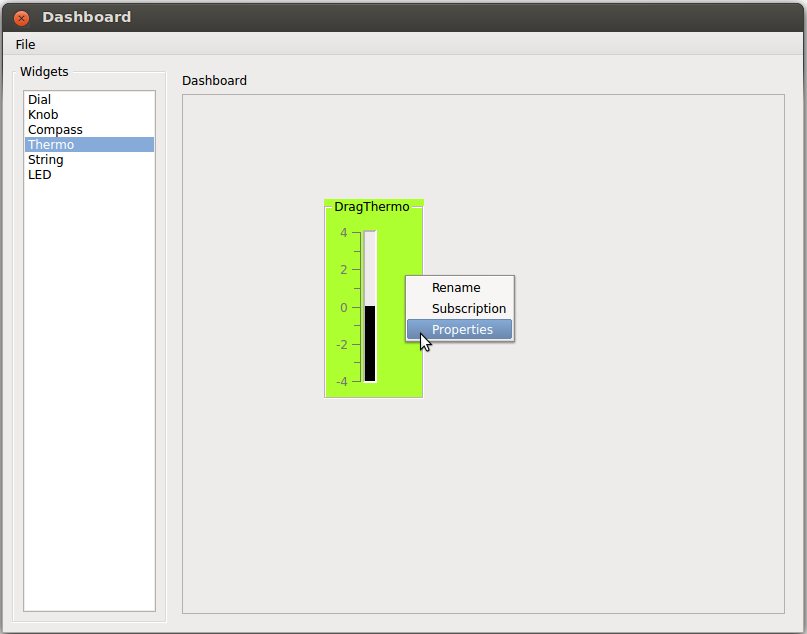
\includegraphics[width=0.45\textwidth]{img/screenflow4.png}
}
\subfigure[Properties dialog]{
    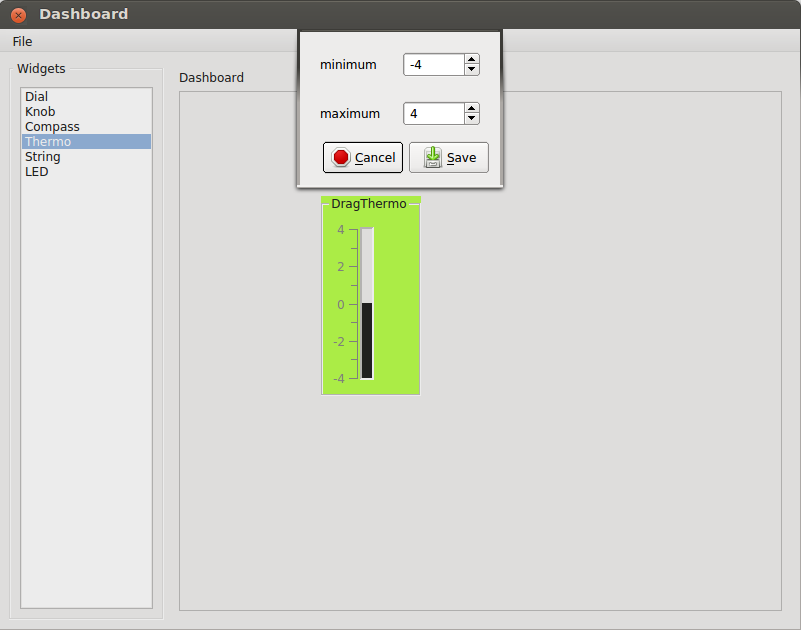
\includegraphics[width=0.45\textwidth]{img/screenflow5.png}
}
\subfigure[Drag to bottom to remove]{
    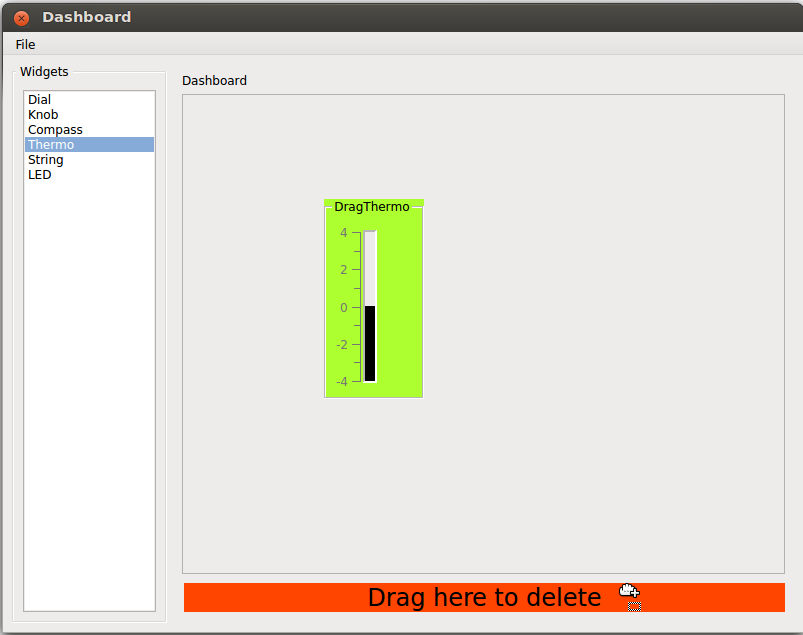
\includegraphics[width=0.45\textwidth]{img/screenflow6.png}
}
\caption{Screenflow when adding and removing widgets from the Dashboard.}
\label{screenflow}
\end{figure}


The widget's background has two different colours to provide additional feedback to the developer whether the visualization is connected to a topic or not. When the configured topic for a visualization widget is not available yet, the background of the widget is coloured in orange. Once the topic becomes available the widget changes its background colour to green. This mechanism only checks the availability of a topic on the communication middleware, it does not time out if a topic has been without any messages for a while. Figure~\ref{colour_widgets} shows the two different colour states of a widget. \enlargethispage{-6em}

\begin{figure}[htb]
  \centering
  \framebox{
    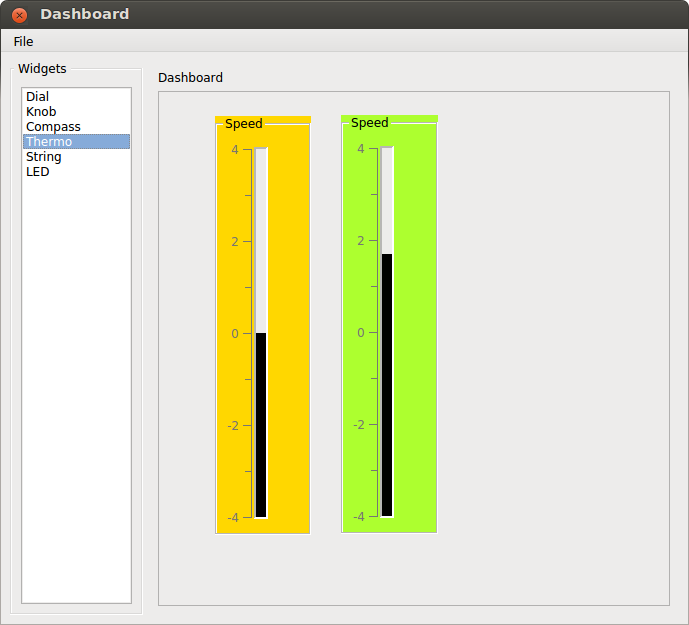
\includegraphics[width=0.6\textwidth]{img/colour_states.png}
  }  
  \caption{Different colour cues provide additional information.}
  \label{colour_widgets}
\end{figure}

\vspace{1em}
Figure~\ref{all_widgets} shows a dashboard with every currently available widget on it. The currently implemented widgets are:

\begin{description}\itemsep4pt \parskip0pt % \parsep0pt \itemsep1pt
\item[Dial] A dial widget similar to the speedometer on the dashboard of a car or motorbike.
\item[Knob] The knob is similar to the dial but is usually smaller. While it is originally often used as input widget, we use it only to visualize numeric data.
\item[Compass] The compass is a 360 degree display which can be used e.g. to visualize orientation.
\item[Thermo] The thermo is a horizontal progress bar with a scale which is similar to a thermometer.
\item[String] The string widget is a text field to show logging messages or other textual information.
\item[LED] The LED widget can visualize boolean data, the LED is either green or red.
\end{description}

\begin{figure}[htb]
  \centering
  \framebox{
    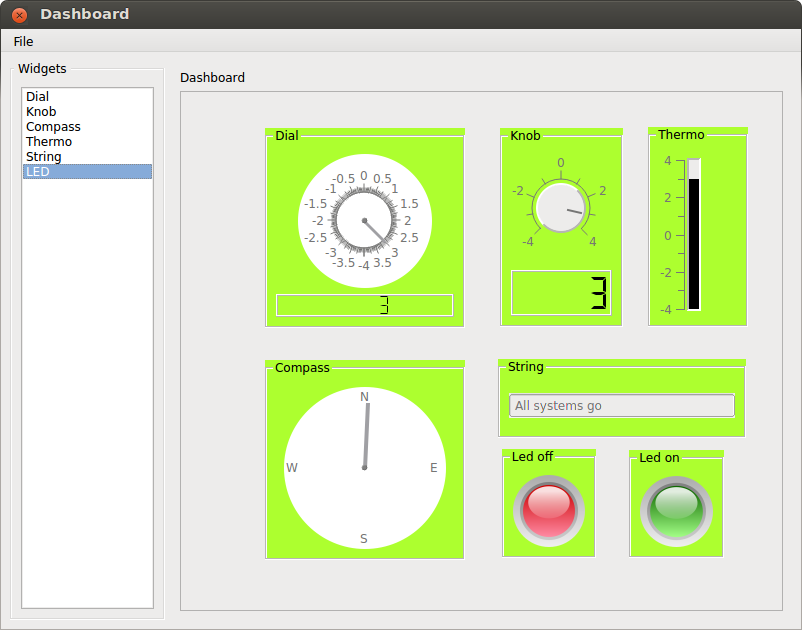
\includegraphics[width=0.8\textwidth]{img/all_widgets_active_screenshot.png}
  }  
  \caption{Dashboard with all currently available widgets.}
  \label{all_widgets}
\end{figure}

\subsection{Data Format}
To share the configuration of a dashboard a save and restore mechanism was integrated. ROSDashboard can save a current configuration of the dashboard to a file which can be used to save the current work and to provide other developers with the same interface. For the prototype all data is stored in a text-based file in JSON (JavaScript Object Notation) \cite{JSON} format. Listing~\ref{json_example} shows an example dashboard configuration represented as JSON, which can be stored in a file. The example contains one visualization widget which is a thermometer widget and is set up to visualize data from the linear field of the \emph{/turtle1/command\_velocity} topic.

\begin{lstlisting}[float,frame=single,caption={Example dashboard configuration in JSON.},label=json_example]
{
  "widgets":[
    {
      "width":105,
      "height":197,
      "name":"Linear Velocity",
      "posX":50,
      "posY":25,
      "subscription":{
        "topic":"/turtle1/command_velocity",
        "datafield":"linear",
        "regex":".*"
      },
      "type":"DragThermo",
      "properties":[
        {
          "type":"numeric",
          "name":"minimum",
          "value":-4
        },
        {
          "type":"numeric",
          "name":"maximum",
          "value":4
        }
      ]
    }
  ]
}
\end{lstlisting}
% \enlargethispage{-4em}

This feature could also be used by robot software and hardware manufacturers to provide a dashboard for a specific module or piece of robot hardware. The dashboard configuration can be made available as part of the module's documentation and represents a easy way to explore the possibilities of a new hardware or software module.


\subsection{API}
\label{api_section}
The current ROS logging framework publishes the log messages on the special purpose topic \emph{/rosout}, but converts everything to a String before the transmission. Since those logging messages are text based, valuable information about the type of the data is lost. To use the data for visualization, the type information must be kept. Thus a set of convenience methods were exposed in the ROSDashboard API (Listing~\ref{api_calls}) to provide a simple interface to publish data for the visualization. The interface is similar to the logging API exposed in the ROS client libraries and basically wraps the ROS specific methods to publish data on a topic. Listing~\ref{api_implementation} shows the simple implementation of the \verb+logint+ API method.

\begin{lstlisting}[float,frame=single,caption={ROSDashboard API methods.},label=api_calls,language=Python,numbers=left,breaklines=true]
# log arbitrary data, try to find the data type with introspection
api.log(tag, data)

# log string message
api.logstring(tag, msg)

# log integer value
api.logint(tag, value, msg_type=Int32)

# log float value
api.logfloat(tag, value, msg_type=Float32)

# log bool value
api.logbool(tag, value)

# log complex data with datatype
api.logdata(tag, data, msg_type)
\end{lstlisting}

\begin{lstlisting}[float,frame=single,caption={Implemented logint API method.},label=api_implementation,language=Python,numbers=left,breaklines=true]
def logint(tag, value, msg_type=std_msgs.msg.Int32):
    """
    publishes a integer value to the /rosdashboard/<tag> topic
    Be careful to use only valid tags, ROS does not allow
    dashes and dots in the topic name.
    
    The default integer message type is std_msg.msg.Int32
    """
    pub = rospy.Publisher('/rosdashboard/' + tag, msg_type)
    pub.publish(msg_type(value))
\end{lstlisting}

The API methods shown in Listing~\ref{api_calls} can be used like logging statements to emit data for visualization. The \verb+TAG+ parameter is used to identify the data when the visualization widgets are set up. Internally the data is published as a message on a ROS topic. The topic name consist of the ROSDashboard specific prefix \emph{/rosdashboard/} and the tag given as parameter. Listing~\ref{example_api_call} shows an example use of the API to publish a integer value with the tag ``proximity''. The value ``17'' will be published on the ROS topic \emph{/rosdashboard/proximity} and can be visualized with a widget in ROSDashboard that points to the respective topic name and accesses the ``data'' datafield of the message.

%fix listing split across pages
%\pagebreak
\vspace{1em}
\begin{lstlisting}[frame=single,caption={Example API usage.},label=example_api_call,language=Python,numbers=left,breaklines=true]
import rosdashboard

rosdashboard.logint('proximity', 17)
\end{lstlisting}

Although this solution proved to be a useful way to expose data during debugging, it might not be feasible for a bigger project because it introduces a new dependency to ROSDashboard. Since the API is only a set of convenience methods that publish data on ROS topics, data can also be published using the same ROS methods the API uses directly in the target application. Other possible solutions will be discussed as future work in Chaper~\ref{future_work}.

